\documentclass[a4paper,12pt]{article}

%% Language and font encodings
\usepackage[english]{babel}
\usepackage[utf8]{inputenc}
\usepackage[T1]{fontenc}

%% Sets page size and margins
\usepackage[a4paper,top=3cm,bottom=2cm,left=2.54cm,right=2.54cm,marginparwidth=1.75cm]{geometry}

\usepackage{graphicx}
\usepackage{amsmath}
\usepackage{csquotes}% Recommended
\usepackage[colorinlistoftodos]{todonotes}
\usepackage[colorlinks=true, allcolors=black]{hyperref}
\usepackage{float}
\usepackage{setspace}
\usepackage{diagbox}

\renewcommand\thesection{\arabic {section}}

\usepackage[style=authoryear-ibid,backend=biber]{biblatex}

\addbibresource{references.bib}% Syntax for version >= 1.2

\begin{document}

%%---------------------------------------------Content---------------------------------------

\clearpage
\tableofcontents\label{c}

\clearpage
\section{Introduction}\label{Introduction}
Identify individuals is important for society. Before the explosion in population growth, people could easily recognize each other by using body characteristics such as face, voice, because thee small communities where they lived in\parencite{Jain:2011bio}.In recent years, identification or authentication system is widely used in website, smart phones, banks and airport to protect us, include our information\parencite{Pinto:2018evolution}. 

The identification or authentication process for machines normally based on three methods: (1) what person knows, (2) what person possess, (3) what person are. While the first method relies on person's knowledge; the second method based on things which only kept by the person, the thing is used like token; the third method depend on the inherent physical signal which is know as biometric. The identification system based on knowledge and token such as using passwords or ID card, can be easily forgotten/lost, guessed/stolen or shared\parencite{Jain:2011bio}. To more specific, password is used in nearly all identification systems, but it is difficult to chose a good password which should satisfy a rule called "easy to remember but hard to guess". As supplementary, 2 - factor authentication is used for many systems to improve security, the second factor is USB-key or ID card. As the discussion before, the main problem for those two factors are the same. they are physical objects which can be easily forgotten/lost, it will cause unexpected deny of service\parencite{Blasco:2018feasibility}.

Biometric recognition is more secure and gives a more reliable solution for person recognition because of the biometric features are unique for every individual\parencite{Jain:2011bio}. Compare with password or ID card, static biometric features such as fingerprints, face, iris; and dynamic features, for instance, voice, PPG(Photoplethysmogram) and ECG(Electrocardiogram), are hard to steal or manipulate\parencite{Agrafioti:2011heart}. In additional, compare with static biometric features, dynamic features can meet more secure needs. Such as liveness detection and continuous authentication\parencite{Agrafioti:2011medical}.

In this paper, we purpose to finding a transfer equation from PPG to ECG, it is a risk from ECG identification system. ECG signals are more considering as sensitive information, which can shows not only personal health information but also psychological status\parencite{Damousis:2008unobtrusive}. Because of that, gathering ECG from individual is difficult and expensive. However, PPG can be easily collect because of the fitness trackers and smart-watches have become very popular\parencite{Blasco:2018feasibility}. Thus, the attack which forge victim's ECG to cheat identification system by transfer from victim's PPG will be much easier and cheaper than collect victim's ECG signal directly. And the risk should be considered seriously. 

The following sections will be organized as: Section 2 will discuss biometric system, include some current attacks, PPG and ECG authentication system and some relevant attacks. Section 3 will cover information on machine learning which include those methods used in authentication system. Neural network will be extract from those method. Section 4 will be some related work.

\section{Biometrics}\label{Biometrics}
Biometrics, or biometric recognition, is becoming more and more popular in government and civilian identity management applications because it is the only way the identity management system can figure out whether the individual is already known or not\parencite{Jain:2011bio}. Biometrics is a pattern recognition problem, user who wants to be authenticated should registered a set of physiological and/or behavioural characteristics before and provides a current characteristics to match the previous one\parencite{Blasco:2018feasibility}. For example, physiological characteristics contain face, iris and the fingerprints, on the other side, keystroke dynamics, gait and voice\parencite{Agrafioti:2011heart}. 

\subsection{Biometric System}
The process in a common Biometric system should like Figure \ref{fig:common_process}.

\begin{figure}[h!]
\centering
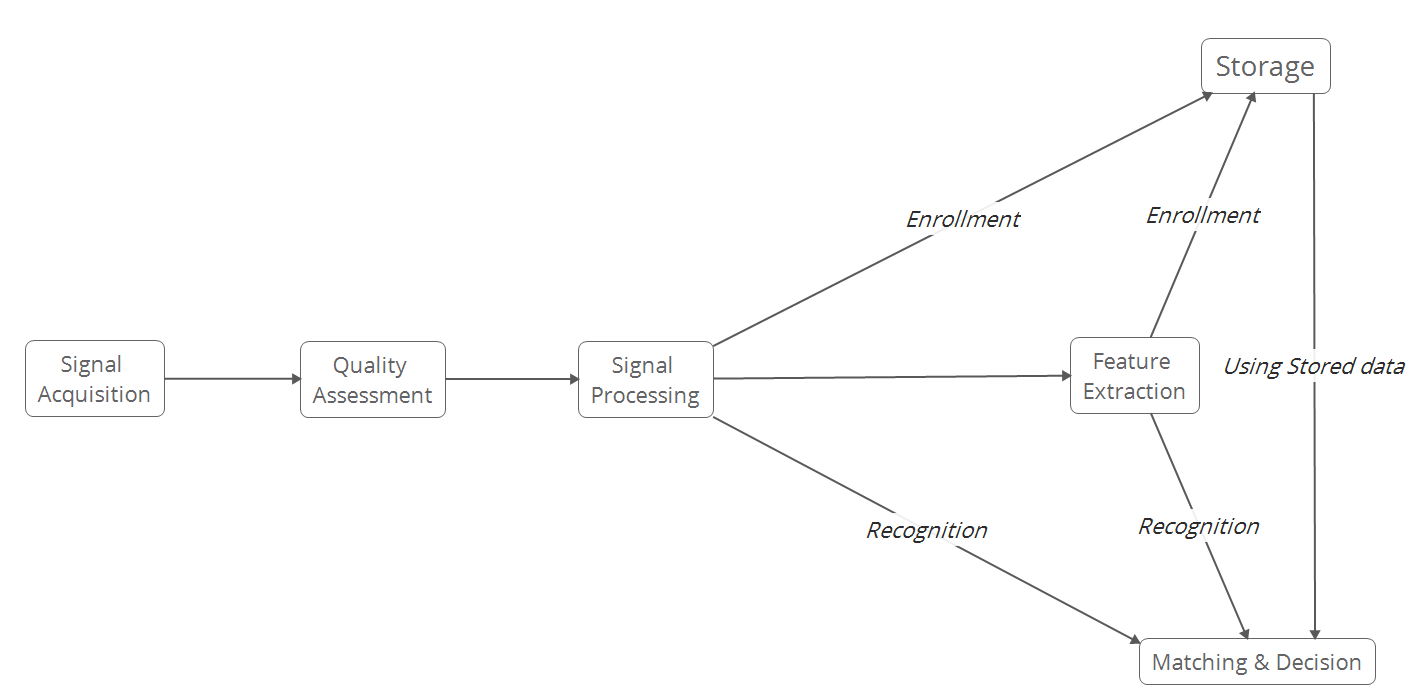
\includegraphics[width = .8\textwidth]{common_bio_process.png}
\caption{The common process for biometric system}
\label{fig:common_process}
\end{figure}



\subsection{Medical Biometric}
\subsection{Current Attacks}

\section{Machine Learning}
\subsection{Machine Learning in Authentication}
\subsection{Neural Network}

\section{Related Work}

\section{Conclusion}

\printbibliography

\end{document}
